\documentclass{sysuthesis}
\usepackage{sysucode}  	% 在论文中使用代码
\usepackage{multirow}

%%
% 论文相关信息
% 本文档中前缀"c-"代表中文版字段, 前缀"e-"代表英文版字段
% modifyer: 黄俊杰(huangjj27, 349373001dc@gmail.com)
% update date: 2017-04-13
%%

% 标题
% 论文题目应以简短、明确的词语恰当概括整个论文的核心内容, 避免使用不常见的缩略词、缩写字。读者通过标题可大致了解毕业设计(论文)的内容、专业的特点和科学的范畴。中文题目一般不宜超过 24 个字,必要时可增加副标题。外文题目一般不宜超过 12 个实词

% 封面标题。由于技术所限,封面题目过长的划分交由用户您进行定夺
% 这也能让您的论文封面看起来更有美感
\covertitlefirst{ 基于远程直接内存访问的 }
\covertitlesecond{ 分布式内存对象存储数据传输优化 }

% Author:   Souler Ou
% 修改者:    欧一锋
% Date:     3/30/2018
% Mail:     ou@souler.cc
%如果英文标题过长可以使用此两项作为表三(答辩记录表)的标题。
\etitlefirst{ Data Transfer Optimization of Distributed }
\etitlesecond{ In-Memory Object Store Using RDMA }

% 中文标题
\ctitle{ 基于远程直接内存访问的分布式内存对象存储数据传输优化 }
\etitle{ Data Transfer Optimization of Distributed In-Memory Object Store Using RDMA }

% 作者详细信息
\author{兰靖}
\cauthor{兰\ 靖}    % 封面作者
\eauthor{Jing Lan}
\studentid{18340085}
\cschool{计算机学院}

\cmajor{计算机科学与技术}
\emajor{Computer Science and Technology}

% 指导老师
\cmentor{肖侬 \ (教授)}
\ementor{Prof. Nong Xiao}     	% 论文相关信息
\input{docs/proposal}   % 开题报告内容
%%
% 摘要信息
% 本文档中前缀"c-"代表中文版字段, 前缀"e-"代表英文版字段
% 摘要内容应概括地反映出本论文的主要内容,主要说明本论文的研究目的、内容、方法、成果和结论。要突出本论文的创造性成果或新见解,不要与引言相 混淆。语言力求精练、准确,以 300—500 字为宜。
% 在摘要的下方另起一行,注明本文的关键词(3—5 个)。关键词是供检索用的主题词条,应采用能覆盖论文主要内容的通用技术词条(参照相应的技术术语 标准)。按词条的外延层次排列(外延大的排在前面)。摘要与关键词应在同一页。
% modifier: 黄俊杰(huangjj27, 349373001dc@gmail.com)
% update date: 2017-04-15
%%

\cabstract{

    % 摘要应概括论文的主要信息,
    % 应具有独立性和自含性,即不阅读论文的全文,就能获得必要的信息。摘要内容一般应包括研究目的、内容、方法、成果和结论,要突出论文的创造性成果或新见解,不要与绪论相混淆。语言力求精练、准确,以300-500字为宜。关键词是供检索用的主题词条,应体现论文特色,具有语义性,在论文中有明确的出处,并应尽量采用《汉语主题词表》或各专业主题词表提供的规范词。关键词与摘要应在同一页,在摘要的下方另起一行注明,一般列3-5个,按词条的外延层次排列(外延大的排在前面)。

    随着大数据处理、大规模智能模型训练、强化学习等多样化、高负载的计算需求成为学术界和产业界的焦点,作为计算基础设施的分布式计算框架(例如Mapreduce, Spark, Ray)
    正在得到更多的关注和更广泛的应用。通常,计算框架软件负责为用户调度计算任务,同时管理和最大限度地利用计算集群的物理资源。
    上述场景所产生的快速增长的计算需求,正在使计算集群的性能愈发捉襟见肘:一方面,高性能计算(HPC)集群正在取代廉价的计算机器以加速高强度计算。值得注意的是,前者所拥有的新型高性能网络,明显地区别于传统集群。
    以智能网卡为硬件基础,高性能计算机能够在无中央处理器(CPU)的介入下,对机器内存直接读写和传输数据。这种被称为远程直接内存访问(RDMA)的传输机制,相比以太网具有低占用、低延迟、高带宽等技术优势。
    另一方面,作为基础设施的软件框架,也在面临严峻的性能挑战。当前大多数分布式计算框架仍然缺乏对高性能硬件的支持,特别是无法充分利用集群中的高速网络资源。
    因此,本研究选取了分布式计算框架Ray的核心组件:分布式内存对象数据库Plasma,首先测试和分析了其使用以太网传输数据而导致的性能瓶颈。然后,在高性能集群上,我们提出了一种支持RDMA特性的高吞吐数据传输机制。
    该机制针对大型数据,提出了基于单边读语义的传输协议,实现了用户态的内存零拷贝。并且该机制能够在运行时,根据数据大小动态地选择传输协议,以获得最佳性能。进一步,我们基于并行计算范式MPI构造了分布式、可扩展的多节点传输性能测试。
    在实验中,我们确定了传输协议选择的最优参数,并且展示了在天河高性能集群上,优化后的内存平台能够在常见大小的对象传输中实现至多8倍的吞吐率提升。

}
% 中文关键词(每个关键词之间用“,”分开,最后一个关键词不打标点符号。)
\ckeywords{数据传输,高性能网络,RDMA,键值对数据库,分布式缓存}

\eabstract{
    % 英文摘要及关键词内容应与中文摘要及关键词内容相同。中英文摘要及其关键词各置一页内。
}
% 英文文关键词(每个关键词之间用,分开, 最后一个关键词不打标点符号。)
\ekeywords{data transfer, high-performance network, RDMA, key-value database, distributed memory}   % 摘要内容
\input{docs/grading}    % 成绩评定记录表评语
\input{docs/progress}   % 过程检查报告数据
\begin{document}
% 论文前置部分
\frontmatter
\pagenumbering{Roman}
\makeUndergraduateCover    	   % 封面
\makeUndergraduateTitlePage    % 扉页
% \makeProposal		  % 开题报告
% \makeProgressCheck  % 过程检查记录表
% \makeDefenseRecord  % 答辩情况等级表
\makedisclaim         % 学术诚信声明
\makeabstract         % 中英文摘要
\maketableofcontents  % 目录
\makelistoffiguretable

% 论文主体部分
\mainmatter
% 引言

% 正文
%%
% 引言或背景
% 引言是论文正文的开端,应包括毕业论文选题的背景、目的和意义;对国内外研究现状和相关领域中已有的研究成果的简要评述;介绍本项研究工作研究设想、研究方法或实验设计、理论依据或实验基础;涉及范围和预期结果等。要求言简意赅,注意不要与摘要雷同或成为摘要的注解。
% modifier: 黄俊杰(huangjj27, 349373001dc@gmail.com)
% update date: 2017-04-15
%%

\chapter{绪论}
% 定义,过去的研究和现在的研究,意义
\label{cha:introduction}
\section{选题背景与意义}
\label{sec:background}
% What is the problem
% why is it interesting and important
% Why is it hards, why do naive approaches fails
% why hasn't it been solved before
% what are the key components of my approach and results, also include any specific limitations,do not repeat the abstract
%contribution
% 引言是论文正文的开端,应包括毕业论文选题的背景、目的和意义;对国内外研究现状和相关领域中已有的研究成果的简要评述;介绍本项研究工作研究设想、研究方法或实验设计、理论依据或实验基础;涉及范围和预期结果等。要求言简意赅,注意不要与摘要雷同或成为摘要的注解。

分布式计算框架是一种复杂的平台软件。传统的并行计算范式如信息传递接口(MPI)和分区全局地址空间(PGAS),通常为编程者提供丰富的调用接口和灵活的编程空间。
然而,使用这些编程标准的门槛过高:编程者通常需要自己管理多台机器的状态,特别是内存的分配和使用;编程者还需要使用给定的标准原语,精确地规定多个进程之间的通信和协作方式,
这通常需要大量时间和精力;另外使用这些范式将导致程序和功能的强耦合——编程者很可能不得不重新编写代码来更新程序的逻辑。因此,现代分布式计算框架通常承担了上述硬件管理的角色,
并针对目标任务类型,为用户设计尽可能少、但简单易用的功能接口,来降低集群的使用难度。传统的分布式计算框架,例如Mapreduce和Spark,都是面向大规模数据分析而设计的。然而,近些年
以强化学习、复杂工作流等为代表的复杂计算需求,需要更灵活的框架支持。加州大学伯克利分校RISELab实验室提出的Ray和芝加哥大学Globus实验室提出的Parsl是其中两个典型。这些框架
吸取了云计算领域“函数即服务(Function as a Service, FaaS)”的设计思想,能够细粒度地以函数为单位将任务调度到集群上执行,同时依然对用户隐藏绝大部分实现细节。Ray通过分布式内存对象存储Plasma,
实现了框架完全自主的集群内存管理,让用户可以专注于实现功能逻辑,无需担心数据的存放和移动。Ray在保持易用性的前提下,极大地提升了计算框架的灵活性,用户只需要修改几行代码就能将单进程程序扩展到整个集群,
进而实现分布式机器学习等复杂模型。

高性能集群(或超算集群),是一种以高端处理器、并行加速卡、高性能网络、大容量存储为核心硬件的计算集群。随着大数据应用的丰富、超大规模人工智能模型的出现,高性能集群和超级计算机正在变得愈发重要。
首先,高性能计算机拥有普通机器不能比拟的计算能力,主要表现为高端的多核处理器和并行加速卡。而随着大模型时代的到来,新应用对集群网络的需求快速提高,高性能网络所表现出的高带宽、低延迟等特性
也逐渐受到了更多的关注。当前,高性能计算集群普遍使用的是英伟达Mellanox子公司的Infiniband高速网络。这一网络架构的性能优势,很大程度上来自于对远程直接内存访问(RDMA)机制的支持。
而对于传统使用套接字(Socket)通信的网络程序,该架构通过“基于Infiniband的互联网协议(IPoIB)”实现支持。值得注意的是,这是一种依赖操作系统内核的非原生支持:已经有多个工作表明,
其网络性能和直接使用RDMA技术相比具有明显差距。然而,要利用RDMA,用户必须在应用中实现基于RDMA的通信机制,而不能依赖于操作系统内核提供的系统调用。
因此,基于Socket的网络应用大多不能在高性能集群中直接获得显著的性能提升。分布式计算框架Ray并不例外,其分布式内存存储Plasma目前仅有对传统TCP/IP协议的支持,因而在超算集群上无法发挥出应有的网络性能,
进而影响Ray运行在超算上的总体性能。

因此,本研究的目的是:我们是否能为分布式内存存储Plasma,提出并实现一种支持RDMA机制的内存通信协议,从而让Plasma乃至整个Ray框架在
现代超算集群上获得更好的性能?从超算研究的趋势来说,应用软件和先进超算硬件之间的隔阂,正在逐渐成为大家关注的热点。随着超级计算机和云计算两个领域的融合,会有越来越多的软件运行在高性能集群中。
然而,它们中的大部分还没有针对高性能硬件提供软件支持——通过提供软件对高性能硬件的支持,我们能够将这些应用的运行性能提升到全新的水平。

\section{国内外研究现状和相关工作}
\label{sec:related_work}

\subsection{分布式计算框架}

分布式计算框架是一种复杂的平台软件。在底层,它通过实现任务调度、并发执行、内存管理等基本组件,向用户透明地提供分布式计算的功能;在应用层,它通过设计和规范一系列接口,帮助用户高效地运行特定任务:例如大数据分析(Mapreduce、Spark),
分布式机器学习(Ray)等等。Ray是近年来最受关注的分布式计算框架,它以函数为单位调度任务执行,完全自主地管理内存移动,并且支持异步执行。借助这一平台,目前社区人员已经实现了机器学习(Ray ML)、强化学习(Ray RLlib)、模型部署(Ray Serve)、工作流(Ray Workflows)
等上层应用库供用户使用。同时,用户也可以直接在框架上编写任意程序:使用常见的Python语法构建出完全分布式的计算程序,而且不会有任何表达能力上的限制。

\begin{lstlisting}[style=sysupython, caption=Ray代码示例]
	import ray
	ray.init()
	
	@ray.remote
	def f(x):
	    return x * x
	
	futures = [f.remote(i) for i in range(4)]
	print(ray.get(futures)) # [0, 1, 4, 9]
\end{lstlisting}

在上述代码片段中,用户通过修饰符"@ray.remote"将函数定义为远程函数,并在下方执行4次。值得注意的是,在Ray框架的调度下,这四次调用将会逐一调度到不同的进程上并发执行,因此Ray能够透明地
为任何函数提供并行计算能力。而分布式内存存储Plasma,则在系统中持续为并发任务调度所需的数据。在示例代码中,Plasma将会在集群中查找变量i的位置,并将其拉取到进程中供任务使用。最后,Ray原生支持异步执行,
任何函数调用都会立刻返回,给予用户一个凭证(future)——用户可以立刻用这一凭证作为参数继续调用其他函数,即使数据的真实值还没有求得。Ray的执行引擎动态地构建和解决数据依赖,将凭证替换为真实值,然后继续调用依赖它的函数。
这一异步特性将使Ray充分发挥并发任务的性能。

\subsection{远程直接内存访问技术(RDMA)}

RDMA全称Remote Direct Memory Access,即远程直接内存访问,是一种于二十一世纪之后逐渐兴起的新型网
络通信技术。其核心思想和直接内存访问(DMA)相似——在早期计算机系统当中,内存读写、移动都需
要由中央处理器(CPU)直接操作,从而带来相当的性能开销。而现代计算机系统分离出了内存子系统,将内
存相关的负载卸载到子系统的专用硬件上。因此,CPU只需要在访问开始和结束时同子系统协作,在漫长的访
问延迟中可以执行其他计算任务,从而大大提高了计算机的总体性能。RDMA技术在这一方向上更进一步:
支持RDMA的现代智能网卡,不仅能从网卡端直接寻址并读写本机内存,还能够和远端的另一个网卡协作,直接读写远端机器的内存空间,
从而实现通信。这一过程中CPU通常只需极少的介入、甚至完全不需要,因此具有相当明显的技术优势:

\begin{enumerate}
	\item 旁路内核(Kernel-bypass)。基于TCP/IP协议的网络通信已经逐渐不能适应现代高并发、重负载的
	网络应用。基于高速SSD的存储系统、基于内存的缓存和(键值对)数据库都需要在短时间内应对大量
	并发的I/O操作请求,工作表明这些应用的性能瓶颈位于CPU,而不是I/O部分。臃肿的网络栈、用户态-内核态的切换、内核态的数据处理和拷贝等等,
	是影响网络系统性能的根本原因。智能网卡能代替CPU执行内存移动,而且CPU和网卡的大多数交互都实现在用户态,大大减轻了CPU的负担。
	\item 零拷贝(Zero-copy)。零拷贝是当前操作系统领域的一项热门技术,其思想在于提高内存的共
	享程度,例如减少进程-进程、用户态-内核态内存拷贝的数量,从而提高I/O的整体性能。在支持RDMA
	的应用中,由于内核旁路,一次内存操作往往能省去:用户缓冲到内核缓冲的拷贝、内核缓冲到硬件
	(驱动)缓冲的拷贝。数据直接在两端主存之间移动,因此产生可观的性能提升。
	\item 低延迟、高并发。简化的网络路径、零拷贝等特性大大降低了机器操作远端内存的延迟。在并发应用中,更低的延迟意味着相同时间内更强大的并发处理能力。
	\item 异步通信。RDMA是原生异步的通信机制,进程需要主动访问完成队列(CQ)甚至直接检查内存数据,才能得知通信的发生。
	这一特性让程序的并发潜力大大提升,但于此同时,编程者需要自己设计同步机制来完成通信,同样增加了编程上的难度。
\end{enumerate}

目前,RDMA技术是智能网卡技术中较为成熟的一种。硬件支持RDMA的网卡通常都具有相当惊人的网络带宽
以及其他诱人的硬件特性:目前,Mellanox NDR Infiniband网卡能够支持高达400Gb/s的网络带宽;另外,
Infiniband标准实现了链路层的容错机制,这意味着通常意义上的丢包在IB网络上并不存在,大大降低
了用户设计通信机制的难度。加上近十年来新型硬件的价格逐渐走低,学术界和工业界争相尝试这一新技术,并
已经有了相当多优秀的成果。尽管RDMA存在着其他实现方式,例如基于以太网的RoCE,但本研究中的RDMA机制在硬件上
基于超算集群中广泛使用的Mellanox Infiniband架构。

基于RDMA机制的网络编程,目前主流的做法是使用Verbs操作原语。在Infiniband网络架构中,两端以队列对(Queue Pair,QP)
\autoref{fig:qp}\footnote{\url{http://hjemmesider.diku.dk/~vinter/CC/Infinibandchap42.pdf}}
为基本模型进行通信,一次简单的发送-接收可以描述为如下步骤:

\begin{figure}[h]
	\centering
	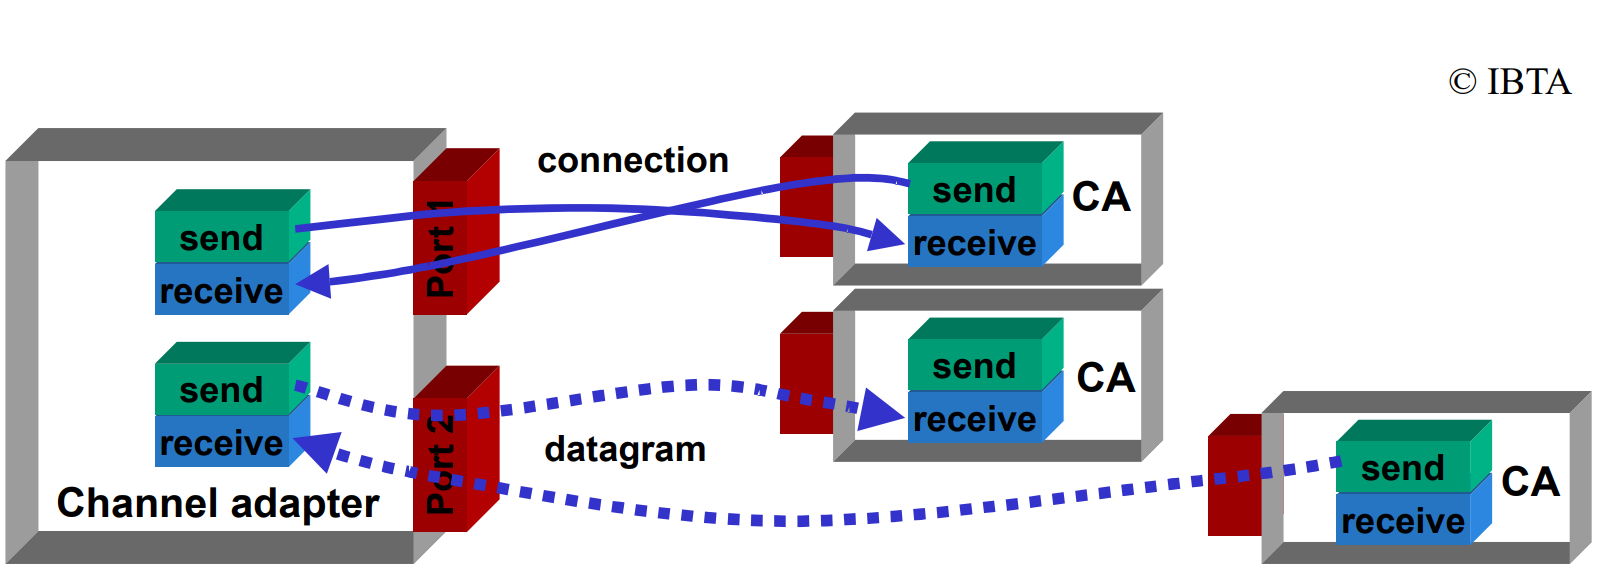
\includegraphics[width=0.6\textwidth]{image/chap01/qp.png}
	\caption{队列对(QP)示意图}
	\label{fig:qp}
\end{figure}

\begin{enumerate}
	\item 两端程序各自创建一个队列对,并借助套接字等基础通信方式,交换队列对的基本信息,建立一对连接。
	\item Infiniband通信的基本单位是一个(发送/接收/完成)事务:接收方通过Verbs调用将一个构造好的接收事务压入到接收队列(Receive Queue)中
	\item 之后发送方将一个构造好的发送事务压入到发送队列(Send Queue)中。
	\item 此时,硬件将为两端处理这一对事务,将本机内存从发送事务指定的内存地址发送到接收事务指定的远端内存地址。
	\item 硬件完成一次事务操作后,通常将一个完成队列项(CQE)压入到完成队列(Completion Queue,CQ)中。
	\item 用户进程可以在任何时刻通过弹出完成队列的头部来确认(发送/接收)事务执行完成,或者得到操作失败的错误代码。
\end{enumerate}

以上流程实现了类似TCP/UDP的双边通信语义,不过,两者仍然有着本质的区别:RDMA通信机制是基于事务模型的;以上操作均在用户态完成,无需任何系统调用;数据从一个进程直接发送到另一个进程。
除此之外,RDMA机制还支持使用读/写(Read/Write)等单边通信语义。在执行这些单边操作时,远端应用不需要事先发送接收事务,也不会通过完成队列得知通信的发生。
使用单边操作语义将会进一步降低远端CPU的介入和负担,从而支持更高强度的并发操作。不过,使用单边语义通常需要引入额外的同步机制以完成通信。

\subsection{基于RDMA技术的内存系统}

近年来,针对RDMA机制提供的高带宽、低延迟优势,研究人员在多个方向上尝试将其转变为实际应用上的性能提升。特别是在RDMA同时支持双边和单边语义的情况下,
如何针对实际应用场景,设计合适的通信和协作机制,一直是这一领域研究的重点。从场景的角度来说,目前的主要研究方向是分布式内存系统和高并发的内存系统。

\subsubsection{分布式内存系统}

Infiniband网络标准和RDMA技术最早应用于高性能计算(HPC)领域。俄亥俄州立大学的\cite{}首次将RDMA技术应用于优化消息传递接口(MPI)的通信机制,这也是最早的、较为完善的一个RDMA
协作机制实现。这一设计针对RDMA单边操作所产生的协作困难问题,预先建立了固定映射的发送-接收缓冲区对,以及设计了自描述的消息块,深刻影响了后续RDMA通信方案的设计。并且在MPI
多年的演进中,其RDMA通信机制也不断有优化方案提出。

然而,从集群内存空间的角度来看,RDMA技术的逐渐成熟,让研究者看到了颠覆性、普适性优化的可能性:优异的访问带宽和极低的访问延迟,已经极大程度地拉近了机器内存之间的“距离”,使得
集群规模的共享内存逐渐成为可能:\cite{}发现IB网络的通信延迟和PCIe总线上的通信延迟处于一个数量级,这说明网络已经不再是集群通信的性能瓶颈。以RDMA为核心,HPC社区和分布式系统社区均
提出了一些分布式共享内存的实现方案,从而以较低的性能代价连接起整个集群的内存空间:前者包括GasNet,OpenSHMEM等支持分区全局地址空间(PGAS)计算的中间件;后者以FaRM,CoRM等系统为代表。
这些研究的共同焦点是分布式的事务机制——除了本地内存的读-写冲突之外,还需要解决远端机器读写和本地访存之间的数据冲突。此外,也有研究避开了细粒度的内存管理,如去中心化、可扩展的
分布式页表系统Infiniswap,就通过粗粒度的内存页交换处理集群中存在的物理内存使用不均的问题。

\subsubsection{高并发内存系统}

在另一个方向上,研究人员希望将RDMA低延迟、高并发的特性直接变为应用的性能——内存键值对(key-value)数据库是一个合适的领域。Redis,Memcached等内存数据库通常被用作一种高速缓存,
其他机器对数据库的访问也主要以并发读取为主,因此非常适合使用RDMA技术进行优化,特别是使用单边读等通信方式优化单机并发能力。不过,基于单边操作的读取机制难以应对高强度并发中的数据冲突问题,
需要借助于更好的哈希函数等其他优化手段才能获得较好的优化效果。因此近期的工作更是提出了双边语义和单边语义混合的通信机制,从而在CPU负载、并发能力和编程难度上都获得较好的结果。
总体来说,在过去的一段时间,针对应用场景不同,研究人员已经提出了众多不同的RDMA通信范式。

\section{论文主要研究内容}

作为分布式计算框架Ray的核心组件,Plasma并没有对RDMA通信的支持,因而在超算集群中存在性能提升的空间。该组件兼有分布式、高并发两方面的特性:
作为集群内存存储,Plasma需要运行在集群的每个计算节点上,并且期望实现最大的并发传输能力,以支撑Ray快速的任务调度。
不过,Plasma并没有实现细粒度的并发机制,而是进一步依靠Redis等外部机制实现。这使得我们的研究重点倾向于优化大型数据对象的传输性能。
在本文中,我们为Plasma提出了一种原生支持RDMA技术的通信机制,并且在现代超算集群上验证了其在各个数据大小的传输上都获得了更优的性能。

这一工作存在以下挑战:

\begin{enumerate}
	\item 目前RDMA编程仍然是极为“小众”的技术,如何能在有限的资料和现有研究帮助下实现高性能的网络通信机制。
	\item 如何在尽可能不破坏项目整体结构的情况下,为Plasma提供原生RDMA通信机制。这要求优化后的程序可以无缝地运行在以太网和Infiniband两种网络架构上。
	\item 针对Ray框架中可能出现的大小不一的数据,如何实现该机制使得Plasma能够在尽可能多的大小范围内都能获得最优的网络性能。
\end{enumerate}

下面总结了本工作的主要贡献:

\begin{enumerate}
	\item 我们通过实验分析了原Plasma实现在超算集群上的存储和网络性能,验证了其无法充分利用Infiniband高速网络,从而证明了使用RDMA技术优化Plasma数据传输的可行性。
	\item 我们针对小对象数据和分布式训练中常见的大对象数据,分别实现了基于双边和单边通信的传输机制。针对大对象,单边通信将实现用户态的零拷贝特性,从而降低了CPU数据拷贝而导致的负载和占用时间。
	\item 我们基于消息传递接口MPI实现了分布式、可扩展的数据传输性能测试,比较了优化实现和原实现在各个数据大小上的性能。并且通过实验,我们确定了机制在选择传输方式时的最佳方案,从而获得了最优的整体性能。
\end{enumerate}

\section{论文结构与章节安排}
\label{sec:arrangement}

本文共分为五章,这些章节的内容安排如下:

第一章:绪论。简述了本文的研究背景和意义,简述了本研究的核心技术背景,并介绍了国内外相关工作和研究现状。

第二章:Plasma分布式内存存储的架构和性能分析。这一章将简要分析Plasma的分布式架构,并且通过性能测试和常见内存存储Redis进行对比,
分析了Plasma在传统网络结构上的性能瓶颈。

第三章:基于RDMA技术的混合通信机制实现。这一章将详细介绍基于RDMA技术的优化方案,并针对大小数据提出混合通信机制的实现。

第四章:实验和分析。这一章将在天河高性能集群上验证优化方案的性能优化,

第五章:总结和展望。这一章将总结本文的主要结果,并且进一步分析后续的工作方向。

\newclearpage
\chapter{Plasma分布式内存存储架构和性能分析}

\section{Plasma架构分析}

Plasma分布式存储架构由多个进程组成。通过将控制面、数据面上的任务解耦到不同的进程,我们可以较为方便地对其软件架构进行改进。
\autoref{fig:plasma_arch}展示了Plasma集群的组织结构。

\begin{figure}[h] 
    \centering
    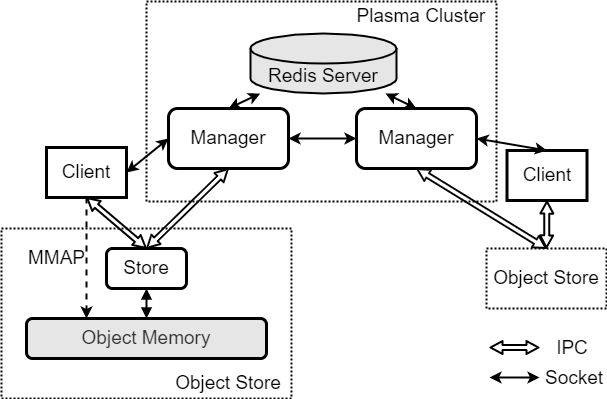
\includegraphics[width=0.75\textwidth]{image/chap02/plasma_arch.png}
    \caption{Plasma存储架构}
    \label{fig:plasma_arch}
\end{figure}

\subsection{Plasma对象存储架构}

对象存储(Object Store)是Plasma运行的最小单元,即Plasma在任意单节点上运行时,可以不需要连接到管理进程(Manager)和Redis数据库。
\autoref{fig:plasma_arch}中左下方部分展示了这一架构。对象存储的基本架构遵循用户端-服务端的特征。Store进程负责直接操作和管理机器内存。
当用户(Client)进程发起创建对象请求时,会将关键元数据——即对象编号(id)、元数据大小、数据大小等通过进程间通信(IPC)发送给Store进程。
值得注意的是,Plasma使用Unix域套接字(Unix Domain Socket)作为进程间通信方式,这一方式允许用户端以类似套接字的方式,通过操作系统内核与本机内的另一个进程交换数据。

Plasma利用MMAP映射机制对内存对象操作进行了性能优化。当前常见的内存数据库如Redis,用户端进程和服务端需要直接交换数据以完成创建、读取等操作。而Plasma利用了MMAP机制,
使得客户端与服务端能够共享内存空间:

\begin{enumerate}
    \item 创建对象时,服务端使用MMAP映射分配内存空间,将其与一临时文件映射。
    \item 服务端通过IPC,将上述临时文件的文件描述符(file descriptor,fd)传递给用户进程。
    \item 用户进程使用相同的文件描述符fd再次调用MMAP。
\end{enumerate}

如此,MMAP向Store进程和用户进程返回同一个内存地址,用户进程能够直接读取、操作数据库中的内存对象。这一架构能够将数据库读取操作的开销
优化到$O(1)$时间复杂度,使Plasma针对大型对象仍然具有优秀的吞吐能力。Plasma在对象存储架构中定义了如下操作原语:

\begin{table}[h]
    \centering
    \caption{Plasma客户端接口}
    \begin{tabular}{*{2}{c}}
        \toprule
        接口定义 & 接口描述      \\
        \midrule
        plasma\_contain(id)                                    & 查询对象是否存在   \\
        buf $\leftarrow$ plasma\_create(id, fields, values)    & 创建参数/数据为fields/values的对象   \\
        plasma\_seal(id)                                       & 封装对象使其对其他进程可见   \\
        plasma\_release(id)                                    & 释放对象,引用计数减一(为0则删除)   \\
        buf $\leftarrow$ plasma\_get(id, fields)               & 读取对象   \\
        plasma\_delete(id)                                     & 删除对象   \\
        \midrule
        plasma\_connect(store\_addr, manager\_addr)            & 连接到Store和Manager \\
        plasma\_subscribe(id)                                  & 等待一个对象在本机被创建 \\ 
        \bottomrule
    \end{tabular}
    \label{tab:store_api}
\end{table}

\subsection{Plasma集群架构}

Plasma存储将其集群架构单独实现为Manager进程,多个进程以及一个Redis数据库共同构成其集群架构,\autoref{fig:plasma_arch}中上方
展示了将Plasma连接成集群的架构。Plasma在集群架构中定义了如下操作原语:

\begin{table}[h]
    \centering
    \caption{Plasma集群接口}
    \begin{tabular}{*{2}{c}}
        \toprule
        接口定义 & 接口描述      \\
        \midrule
        buflist $\leftarrow$ plasma\_fetch(ids)               & 将id列表中的对象拉取到本地存储   \\
        \bottomrule
    \end{tabular}
    \label{tab:manager_api}
\end{table}

管理者(Manager)进程仅处理用户进程发出的一种请求,即输入一个id列表,执行一次拉取(fetch)操作:

\begin{enumerate}
    \item Manager对列表中的每个id,从集群中查找对应数据对象的位置。 
    \item 本地Manager与存有这一对象的另一个Manager建立连接,拉取数据。
    \item Manager和Store交互将数据保存到本地——对Store进程来说,Manager只是普通的Client进程。
\end{enumerate}

在这一过程中,Plasma依赖于Redis提供的数据库服务。每当Client进程创建并封装数据对象时,它将借助Manager与Redis服务器建立通信,并更新该对象在集群中的分布。
因此Manager在拉取数据的过程中(上述步骤2),必须先从Redis得到数据分布,才能开始一次数据传输。

\section{基于套接字的Plasma通信机制}

Plasma实现了基于套接字(Socket)的数据传输机制。通过访问Redis服务器获得对象处在的目标节点后,Manager会逐一尝试建立套接字连接,并拉取数据。
其通信机制如\autoref{fig:sock_protocol}所示:

\begin{figure}[h] 
    \centering
    
\includegraphics[width=0.75\textwidth]{image/chap02/sock_protocol.png}
    \caption{基于套接字的Plasma通信机制}
    \label{fig:sock_protocol}
\end{figure}

发起者(Receiver)首先将一条类别为PLASMA\_TRANSFER的消息发送给存有数据对象的Manager进程。在得知需要发送的对象id后,发送方通过向Store调用查询操作获得了
数据的缓冲区地址。需要注意的是Plasma的读取操作具有常数的时间复杂度,因而会马上返回。发送方(Sender)会将查询到的元数据(主要是数据大小)通过PLASMA\_DATA消息返回给接收方,接收方便会
向Store创建一个同id的对象,获得分配的内存空间。最后双方分别进入发送/接收函数,分批将数据转移到本地缓冲区中。

在Plasma实现中,默认一次发送4kb大小的数据。

\section{Plasma存储和传输基准测试}

为了分析Plasma存储运行在超算上存在的性能瓶颈,得到可能的优化方向,我们在天河高性能集群上对Redis和Plasma进行了存储和传输数据的性能测试。
通信性能测试以IPoIB机制运行在两节点的Mellanox Infiniband网卡上。

\subsection{存储性能测试}

\begin{figure}[h]
    \begin{subfigure}{0.33\textwidth}
        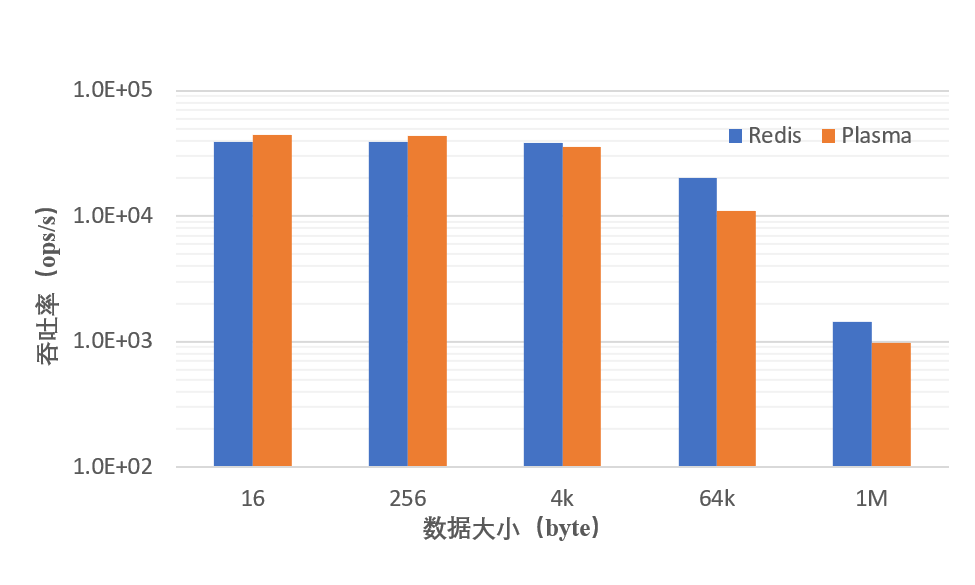
\includegraphics[width=\textwidth]{image/chap02/set.png}
        \caption{Put}
    \end{subfigure}
    \begin{subfigure}{0.33\textwidth}
        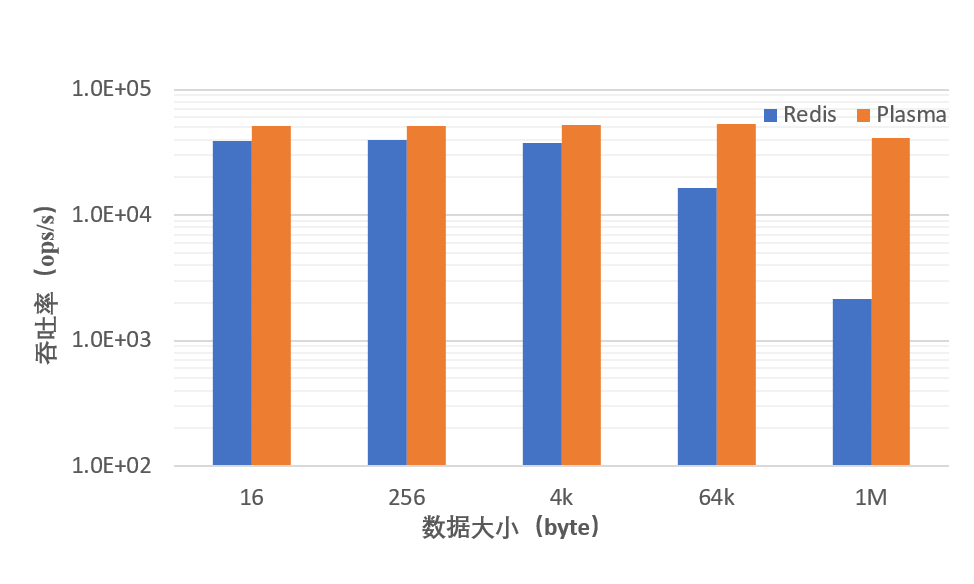
\includegraphics[width=\textwidth]{image/chap02/get.png}
        \caption{Get}
    \end{subfigure}
    \begin{subfigure}{0.33\textwidth}
        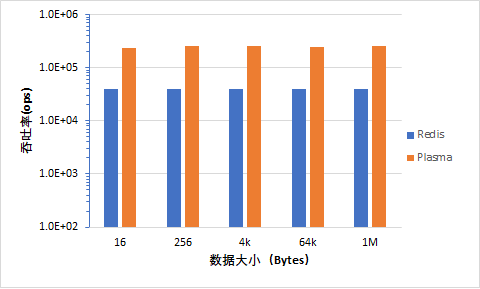
\includegraphics[width=\textwidth]{image/chap02/del.png}
        \caption{Delete}
    \end{subfigure}
    \caption{Redis和Plasma常见操作吞吐对比}
    \label{fig:local_bench}
\end{figure}

如\autoref{fig:local_bench}所示,Plasma单机存储架构的综合性能优于Redis。Plasma和Redis的“put”操作并不相同:对于前者,这一语义实际上是用户通过
调用创建(Create)操作一段分配内存空间,然后将数据对象拷贝到该空间,最终释放(Release)并封装(Seal)对象。可以看到,由于复杂的处理过程,
Plasma在这一操作上有稍高的延迟。由于Plasma通过MMAP机制,在读取操作上支持了零拷贝特性,用户仅需通过IPC接收固定大小的文件描述符,因而在任何数据大小上都具有相似的性能。
相反,Redis使用IPC传输实际数据给用户进程。因此随着数据量增大到1M,Plasma将对Redis有20倍的性能优势。Plasma和Redis在删除上均拥有常数时间复杂度。

\subsection{数据传输测试}

进一步,我们在两个高性能节点上测试了Plasma和Redis在跨节点数据传输上的吞吐能力。对于Redis,我们在远端节点启动Redis服务器,然后在本地基准测试中重复调用Get操作
进行测试。对于Plasma,在远端节点创建多个数据对象,然后在本地节点调用拉取(Fetch)操作。

\begin{figure}[h]
    \centering
    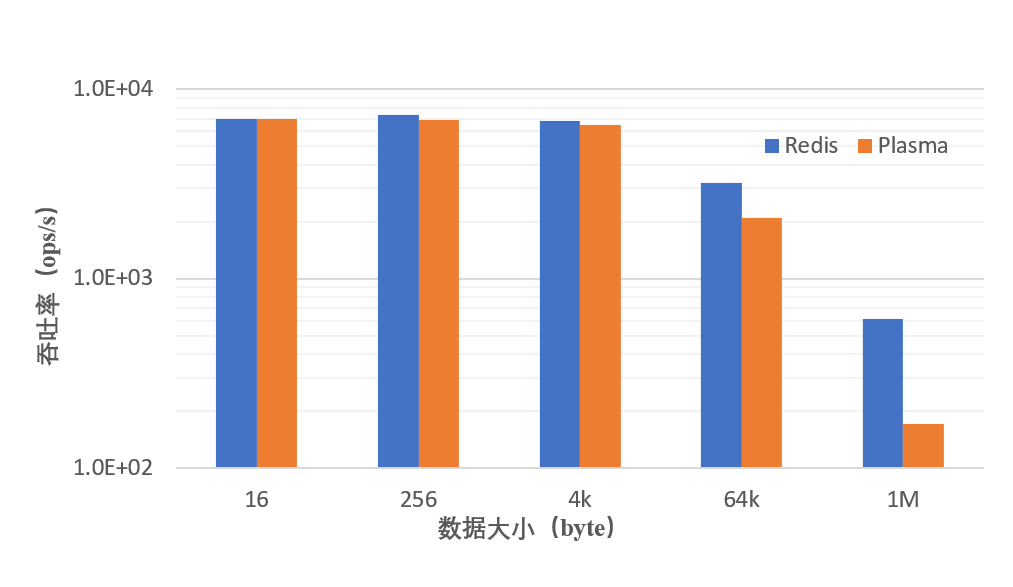
\includegraphics[width=0.7\textwidth]{image/chap02/fetch.png}
    \caption{Redis和Plasma数据传输吞吐对比}
    \label{fig:remote_bench}
\end{figure}

如\autoref{fig:remote_bench}所示,Plasma在远程操作上的吞吐能力比较显著地劣于Redis,在1M大小数据上前者有3.6倍的传输延迟。虽然,两者实际完成的语义很不相同——
Plasma需要先获取对象在集群中的位置,这本身就将访问一次Redis服务器。另外,Plasma发起一次拉取操作包含了一次本地Create操作,也将产生额外的延迟。而且,
Plasma一次仅以4kb为单位传输数据,也是大数据上传输性能明显不如Redis的原因。然而,从我们的实验结果总结来看,不论是Redis还是Plasma都存在明显的性能提升空间:
它们均不能很好地利用超算网络的低延迟和高带宽。特别是支撑分布式计算框架的Plasma,在较大数据的传输上具有明显的性能劣势,这是原实现没有解决的问题。因此,
这一观察促使我们基于超算网络对Plasma的数据传输机制进行针对性优化。
\newclearpage
\chapter{基于RDMA的数据传输机制实现}


\newclearpage
\chapter{性能测试与结果分析}

\section{实验环境配置}

本段将简单介绍运行Plasma的必要环境配置。这包括进行性能测试的集群硬件配置,以及编译、运行Plasma所需的其他软件要求。

\subsection{天河高性能集群硬件简介}

运行测试的天河高性能集群有超过100台CPU服务器,并由100GB的Infiniband高速网络连接而成。每个CPU节点的关键配置如下所示:

\begin{table}[h]
    \centering
    \caption{天河CPU服务器硬件配置}
    \begin{tabular}{*{4}{c}}
        \toprule
        硬件组件  & 数量 & 硬件型号 & 参数配置 \\
        \midrule
        CPU  	 & 2  & Intel(R) Xeon(R) Gold 6150 & \makecell{18核 @2.7GHz \\ L1 Cache 64K \\ L2 Cache 1024K \\ L3 Cache 25344K} \\
        \midrule
        内存 	 & 12 & / & \makecell{16Gb DDR4 \\ with ECC} \\
        \midrule
    	以太网卡 & 1  & Mellanox MT27710 Family [ConnectX-4 Lx]   & 25Gb/s \\
    	IB网卡   & 1  & Mellanox MT27700 Family [ConnectX-4] & 100Gb/s \\
        \bottomrule
    \end{tabular}
    \label{tab:hardware_config}
\end{table}

每个CPU服务器配备有双路Intel至强金牌处理器。每个CPU为6通道16G内存,因此每节点内存总量为192Gb。两路处理器形成两个NUMA节点,每节点上分别挂载有一张网卡。
该型服务器的硬件拓扑图如\autoref{fig:server_block}所示。

\begin{figure}[h]
	\centering
	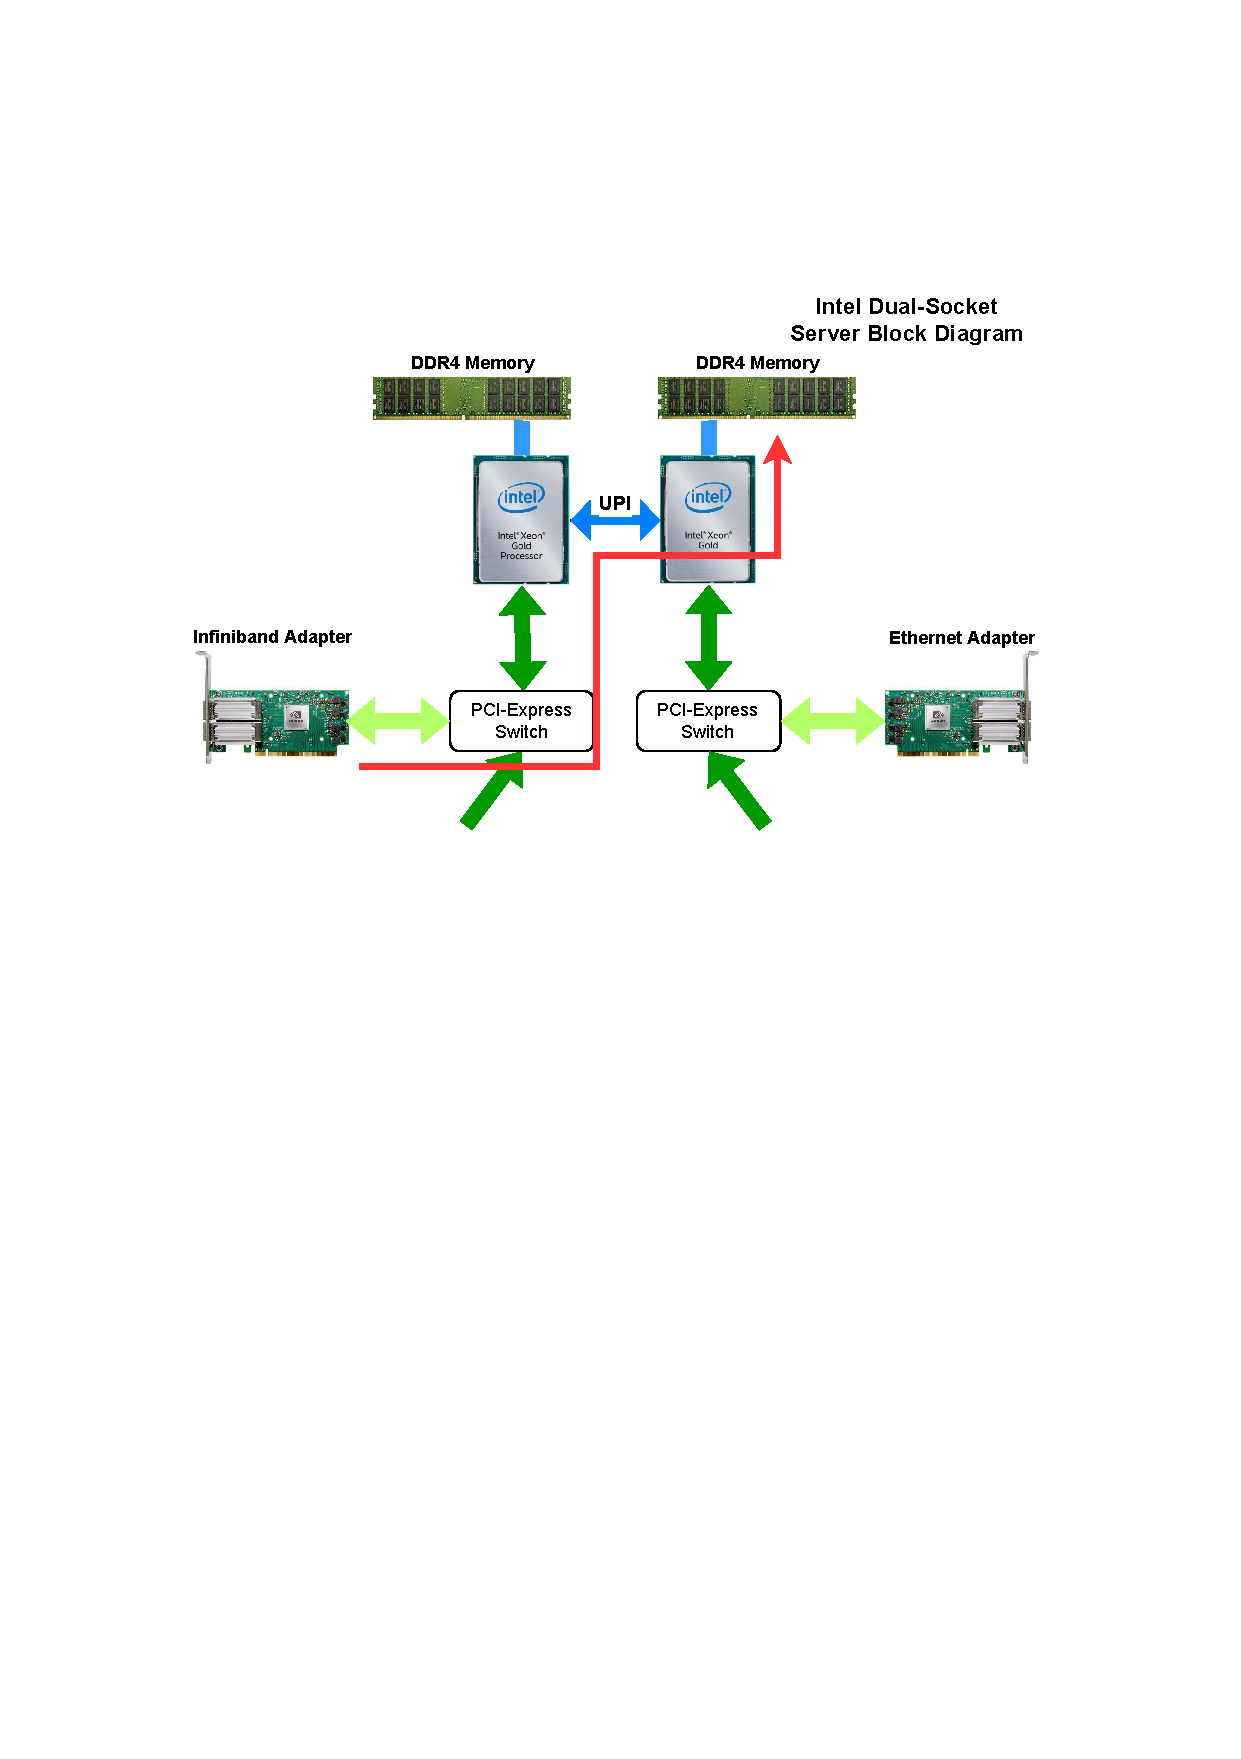
\includegraphics[width=0.8\textwidth]{image/chap04/server_block.pdf}
	\caption{天河CPU服务器硬件拓扑}
	\label{fig:server_block}
\end{figure}

需要注意的是,以太网卡和IB网卡分别挂在两个CPU的PCIe Switch上,因而IB网卡只有在访问本NUMA节点的一半内存时拥有最佳性能——而访问远离它的CPU所控制的一半内存将会有
较大的性能损耗(\autoref{fig:server_block}中间访存路线)。这一特性对基于RDMA的网络通信性能有明显的影响,因此在实验中需要相应调整运行配置。

\subsection{软件环境简介}

\autoref{tab:software_config}展示了本章节各性能测试所运行的软件环境。操作系统一栏展示了天河高性能集群使用的Linux操作系统版本;软件依赖指的是成功编译出可正常执行
的Plasma程序所需要的前置软件;测试软件则表示为了编译基准测试程序、运行测试程序所需要的前置软件。所有软件均使用包管理器spack\cite{gamblin2015spack}安装和管理,
软件名后的数字串表示这些软件在测试时使用的版本。

\begin{table}[h]
    \centering
    \caption{天河CPU服务器软件环境}
    \begin{tabular}{*{3}{c}}
        \toprule
        软件类型 & 软件名称  & 作用描述 \\
        \midrule
        操作系统 & CentOS Linux 7 & Linux内核版本3.10.0-957.el7.x86\_64 \\
        \midrule
        包管理器 & spack@0.16.3 & 安装和管理下述软件依赖 \\
        \midrule
        \multirow{3}{*}{软件依赖} & Redis@3.2.3 & \makecell{Redis服务器存放对象在Plasma集群的分布 \\ ae事件循环库驱动Plasma进程} \\
    	 & \makecell{uthash \\ utlist \\ utarray \\ utstring}@2.0.1 & \makecell{基于宏的C语言头文件库,\\ 封装了哈希表等高级数据结构} \\
		 & gcc@9.3.0 & 编译Redis和Plasma \\
        \midrule
    	\multirow{2}{*}{测试软件} & openmpi@4.1.1 & 编译基于MPI的多节点性能测试 \\
		& hwloc@2.5.0 & 查看服务器的NUMA拓扑结构 \\
		& numactl@2.0.14 & 运行时绑定MPI进程和NUMA节点 \\
        \bottomrule
    \end{tabular}
    \label{tab:software_config}
\end{table}

\section{NUMA架构下的Plasma存储测试}

\textbf{跨NUMA节点访存对性能测试的影响:}上一章节中提到了天河高性能集群存在的NUMA访问架构。IB网卡在NUMA架构中,对“远端”CPU所管理的内存发起内存访问需要通过两个CPU之间的UPI互联(The Intel Ultra Path Interconnect,\autoref{fig:server_block}中间蓝色连接),
因而无法获得最优的访存延迟和带宽,对Plasma本地存储的性能产生较大的不利影响。由于Plasma传输数据前首先会(在发送端)访问或者(在接收端)创建内存对象,因而会进一步影响Plasma跨节点数据传输的延迟和吞吐能力。
所以,为了获得最佳的传输测试结果,我们将首先通过简单的NUMA绑定以优化Plasma的本地存储性能。

在天河高性能服务器中,通过hwloc软件提供的lstopo命令可以查看IB网卡在服务器NUMA架构中所处在的位置:以太网卡挂载在NUMA节点0上,而IB网卡挂载在NUMA节点1上。
这样,我们能通过numactl命令限制plasma\_store和plasma\_manager进程只运行在NUMA节点1,从而避免IB网卡的跨NUMA节点访存。

\textbf{NUMA绑定的性能测试:}为了展示NUMA绑定对访存性能的影响,我们分别在绑定与未绑定的情况下测试了Plasma本地存储操作的性能,同时也对Redis进行测试作为参考。结果如\autoref{fig:numa}所示。很显然,不论是本地读还是本地写
绑定后Plasma的程序性能都有了相当明显的提升:可以看到,在写入较小对象时,绑定的Plasma进程可以获得1.5倍的吞吐能力;不过,绑定运行时的写入性能随着数据增大逐渐下降,
最后和不绑定时持平。在读取和删除对象操作上,绑定NUMA节点在所有数据大小上都有显著的优化效果,其中读取操作的吞吐率增加到原来的至多1.55倍,删除操作的吞吐率增加到原来的至多5倍。

\begin{figure}[h]
    \begin{subfigure}{0.49\textwidth}
        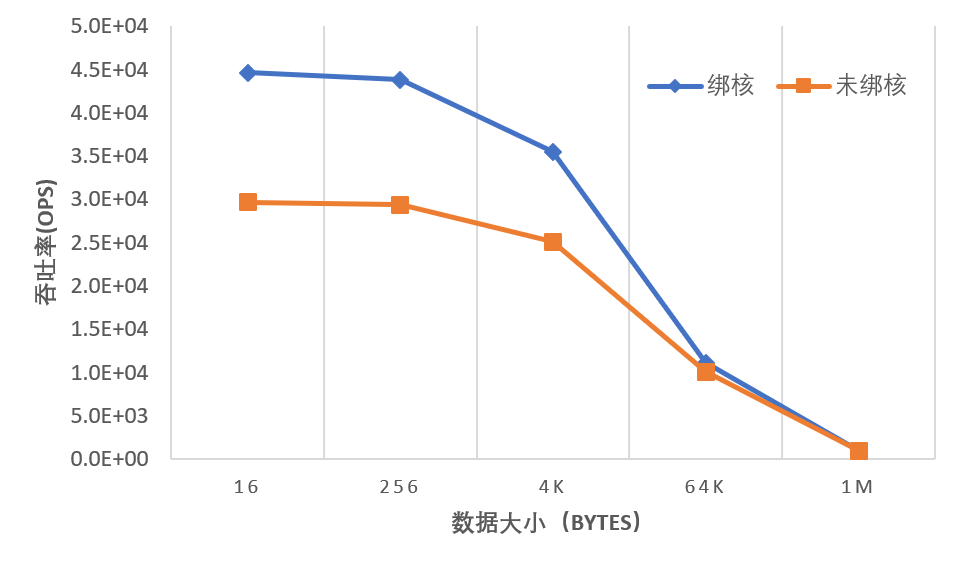
\includegraphics[width=\textwidth]{image/chap04/put.png}
        \caption{Put}
    \end{subfigure}
    \begin{subfigure}{0.49\textwidth}
        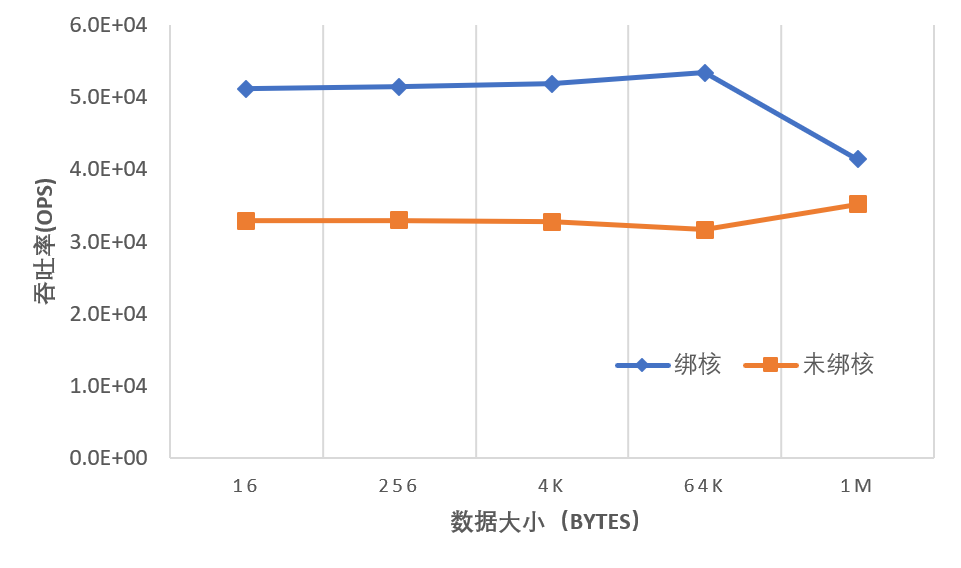
\includegraphics[width=\textwidth]{image/chap04/get.png}
        \caption{Get}
    \end{subfigure}
	\\
	\centering
    \begin{subfigure}{0.5\textwidth}
        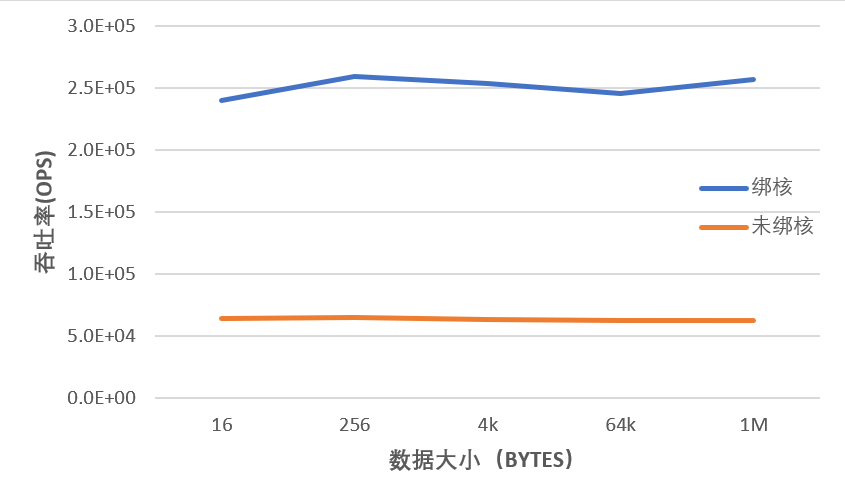
\includegraphics[width=\textwidth]{image/chap04/del.png}
        \caption{Delete}
    \end{subfigure}
    \caption{绑定对Plasma常见操作吞吐率的影响}
    \label{fig:numa}
\end{figure}

与之相比,绑定并不能给Redis带来更强大的吞吐能力——不论是否绑定,Redis在三种常见操作上具有相近的吞吐能力;且在读取/删除操作中,Plasma性能显著更优。
这种区别很有可能是Redis和Plasma传输数据的实现方式不同而导致的:
\begin{itemize}
    \item 如\autoref{sec:plasma_arch}所述,Plasma使用mmap机制获取对象地址后,使用用户态内存拷贝(如memcpy)进行数据读写。
    \item Redis使用的是TCP环回地址(127.0.0.1)向服务器读写数据。
\end{itemize}
Redis在访存上更依赖于操作系统,因此控制Redis进程的NUMA绑定并不会得到明显的性能提升。

由于本地访存的延迟大大降低,且Plasma对象传输过程包括了本地访存操作,因此绑定情况下的多节点传输测试更能够体现出基于RDMA的网络协议在传输性能上的优势。
在之后的性能测试中,基于套接字以及RDMA的传输协议都将运行在一个NUMA节点上。

\section{Plasma网络协议测试}

针对Plasma通过以太网络传输数据所导致的性能瓶颈,我们设计了原生支持RDMA通信机制的数据传输协议。针对可能出现的小对象($\leq 4KB$),我们设计了使用预注册缓冲区的双边通信协议;并且,针对可能出现的大对象($\geq 1MB$),
设计了具有完全零拷贝特性的单边传输协议。因此,优化的Plasma通过混合两种机制,能在不同大小的数据都取得较好的吞吐能力。在Plasma优化实现的性能测试中,我们将测试基于IPoIB的套接字、RDMA双边通信以及单边通信在各个数据大小
上的传输性能,一方面验证RDMA机制在性能上的优越性,另一方面可以确定混合机制的关键决策阈值,从而获得最佳的综合性能。

\textbf{性能测试案例的实现:}我们实现了基于MPI编程范式的多进程网络性能测试。该测试能够在一次运行中对Plasma内存存储的主要操作(本地创建/读取/删除和远程读取)进行性能测量。
该测试采用主-从架构,能够支持任意多从进程并发传输的测试。其流程如下所示:

\begin{enumerate}
	\item (0号)主进程阻塞在MPI\_Barrier处,等待(编号为正整数的)从进程创建数据对象。
	\item 其他进程创建一批数据对象。如果进程编号为N-1,测试Plasma本地操作的性能并输出到日志。
	\item 所有进程在MPI\_Barrier处同步。之后,主进程通过MPI\_Gather接口,从其他MPI进程处汇集所有内存对象的标识符。
	\item 主进程以随机顺序向其他进程处发送plasma\_fetch请求,拉取所有数据对象。
\end{enumerate}

\textbf{小对象传输性能:}在天河高性能集群上,我们对N=2,即点对点拉取数据的情况进行性能测试。如\autoref{fig:small}所示,基于双边通信(IB Send/Recv)的传输协议在16K字节范围内的具有最好的传输性能:协议在该数据范围内的传输延迟,
相较基于IPoIB的套接字协议和使用单边通信(IB Read)的协议,均有20微秒的延迟优势。在这一大小范围内,基于IPoIB的套接字协议和使用单边通信的传输协议性能相当——因此后者同样对双边通信协议具有显著的性能差距。这一结果验证了
我们在\autoref{cha:implementation}中的性能分析:即在较小数据的传输中,使用预注册的内存缓冲区和一次用户态的内存拷贝,相比重复注册内存缓冲区具有更小的时间开销,因而是更好的策略。

\begin{figure}[h]
	\centering
	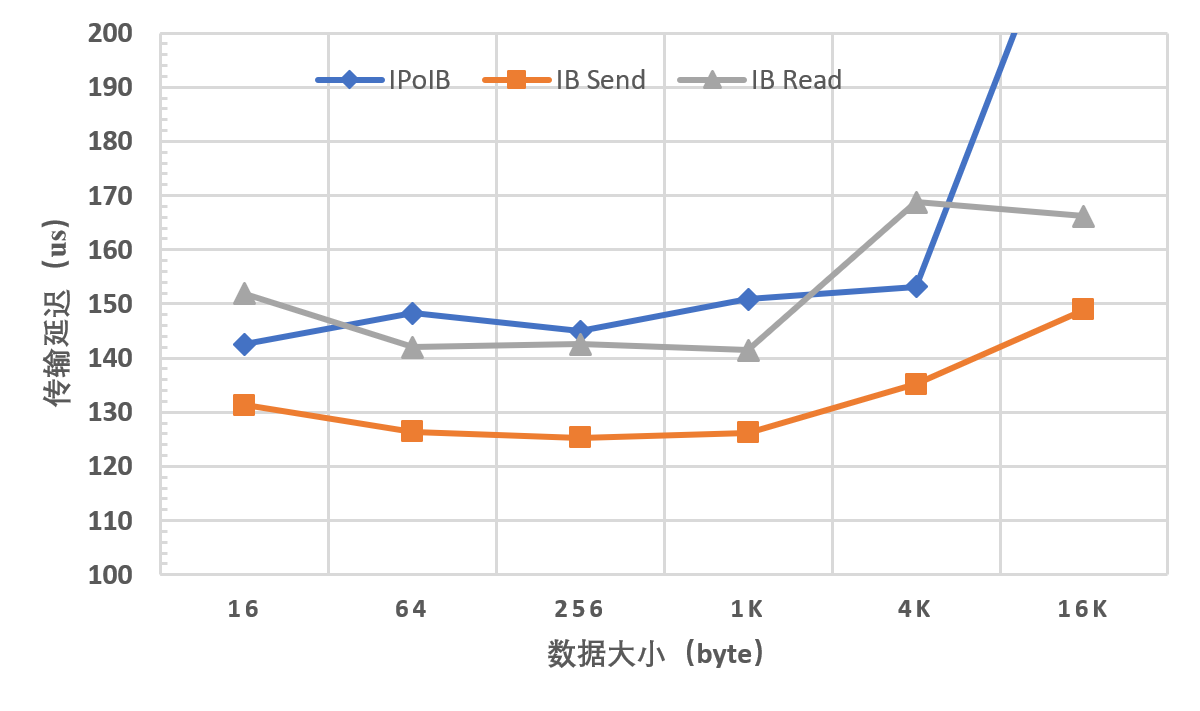
\includegraphics[width=0.9\textwidth]{image/chap04/small.png}
	\caption{三种机制在小对象上的传输延迟}
	\label{fig:small}
\end{figure}

\textbf{大对象传输性能:}并且,上述性能对比在大于16K字节的数据传输中得到了相反的结果,进一步验证了我们对实现的分析。如\autoref{fig:big}所示,原Plasma实现采用的基于IPoIB支持的套接字协议,在每次传输的对象大小大于4K时传输延迟开始快速上升。与之相比的是,随着数据量逐渐增加,使用RDMA机制的传输表现出了更好的扩展性:
不论是基于RDMA的双边通信还是单边通信的传输协议,都表现出了明显的性能优势。使用套接字协议传输1M字节大小的内存对象,RDMA双边传输协议可以在相似时间内传输四倍大小的数据量。进一步,在这一大小范围内,使用RDMA单边读的传输协议,对使用双边通信的传输协议也具有明显的性能优势。
当对象大小大于16K字节时,前者表现出更优的传输延迟,并且该优势随着数据量增大而显著增大——在4M字节的对象传输中,使用单边RDMA操作能将吞吐率再增加一倍。在这一数据大小上,RDMA的较优通信方案表现出了7倍于原实现的传输性能。

\begin{figure}[h]
	\centering
	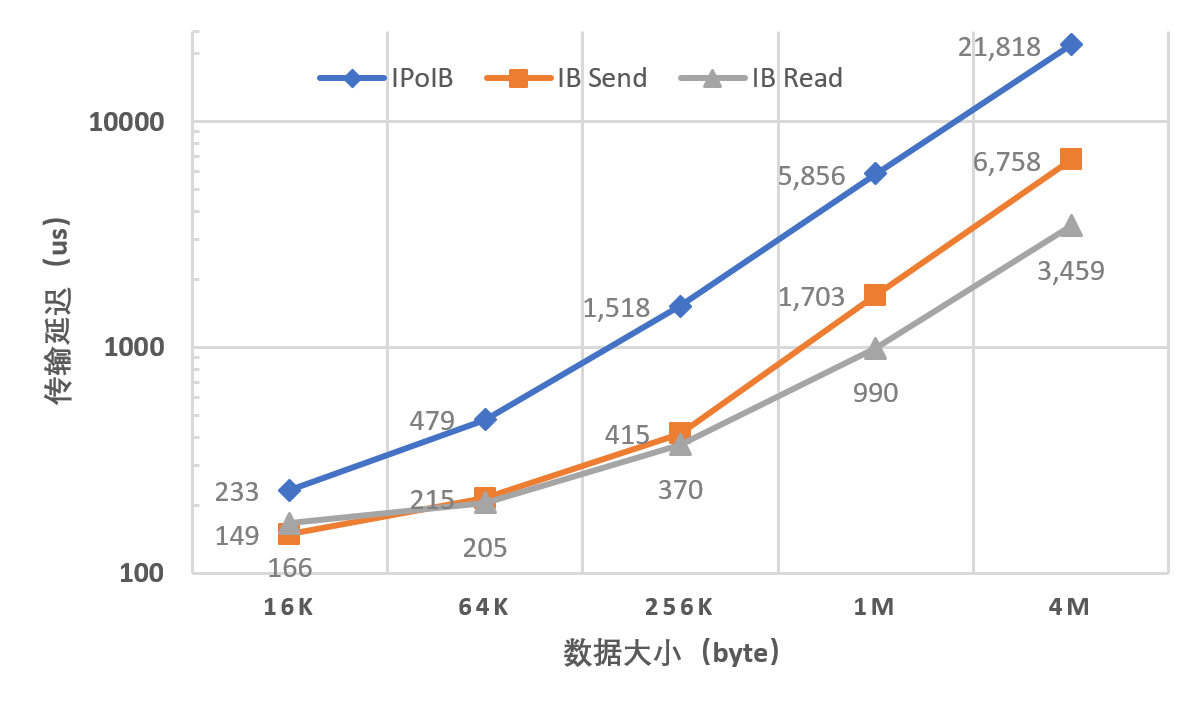
\includegraphics[width=0.9\textwidth]{image/chap04/big.png}
	\caption{三种机制在大对象上的传输延迟}
	\label{fig:big}
\end{figure}

\textbf{混合机制的选择:}上述性能测试在各个常见的数据范围内,展示了原生RDMA机制对传统套接字通信的性能优势。并且,在\autoref{cha:implementation}中我们实现了两种通信协议,并分析了它们的预期性能特征——这一讨论在实验中也得到了充分验证。为了让Plasma能在各个数据范围内充分利用RDMA机制的性能优势,
我们通过观察实验数据,选择常量IB\_READ\_MIN\_SIZE的值为32KB。以该常量值为分界线,当对象大小小于该值时使用双边传输协议,反之使用单边传输协议。此时,我们能够将两种机制的性能特征简单而有效地结合起来,从而达到Plasma实现的最大优化。值得注意的是,最优的参数应当随着CPU、IB网卡、内存等硬件的性能发生变动。
不过,通过我们在本研究中实现的性能测试程序,确定最优的策略应该是容易的。

\textbf{Plasma(优化后)与Redis对比:}在确认了Plasma最佳的混合传输策略之后,我们可以将优化的Plasma实现和Redis作性能对比。两者传输各个大小数据的延迟如\autoref{fig:redis_small}和\autoref{fig:redis_big}所示。
和\autoref{sec:bench}不同,经过RDMA传输优化后的Plasma,已经能在常见大小的对象传输上获得比Redis
显著更优的性能。然而还需要强调的是,Plasma在传输测试中所完成的操作,要比Redis更多——Plasma每次拉取对象到本地内存中,都会创建该对象的一个副本:分配相同大小的内存空间、拷贝数据并且封存;而Redis在性能测试中并不会这么做。总结来说,这是Plasma为了支持Ray分布式缓存、分布式访问所需的额外代价。
然而,通过借助RDMA的硬件优势,我们优化了Plasma内存存储的传输机制,使其在高性能集群上同时拥有了以下技术优势:

\begin{enumerate}
    \item Plasma对象存储具有分布式、可扩展的功能特性:在完成对象数据传输后,Plasma会将其保存为本地副本,从而很好地支持多节点并发访问。
    在功能上,我们实现的Plasma相比Redis更能满足计算框架对数据管理和访问的需求。
    \item 我们优化的Plasma实现具有低延迟的性能特性:即便实现了分布式内存对象存储,Plasma在跨节点数据访问上的延迟仍然显著地低于Redis数据库。
\end{enumerate}

\begin{figure}[h]
	\centering
	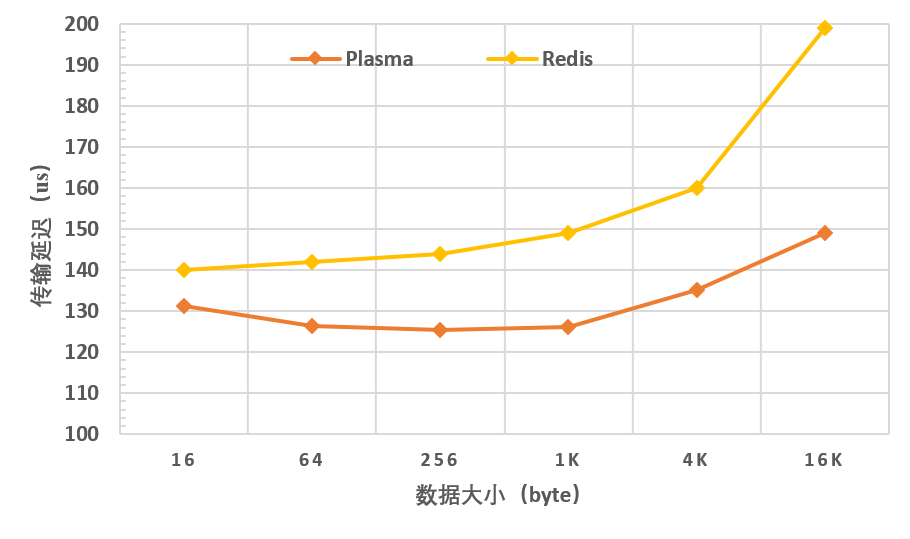
\includegraphics[width=0.9\textwidth]{image/chap04/redis_small.png}
	\caption{Redis和Plasma(优化后)在小对象上的传输延迟}
	\label{fig:redis_small}
\end{figure}

\begin{figure}[h]
	\centering
	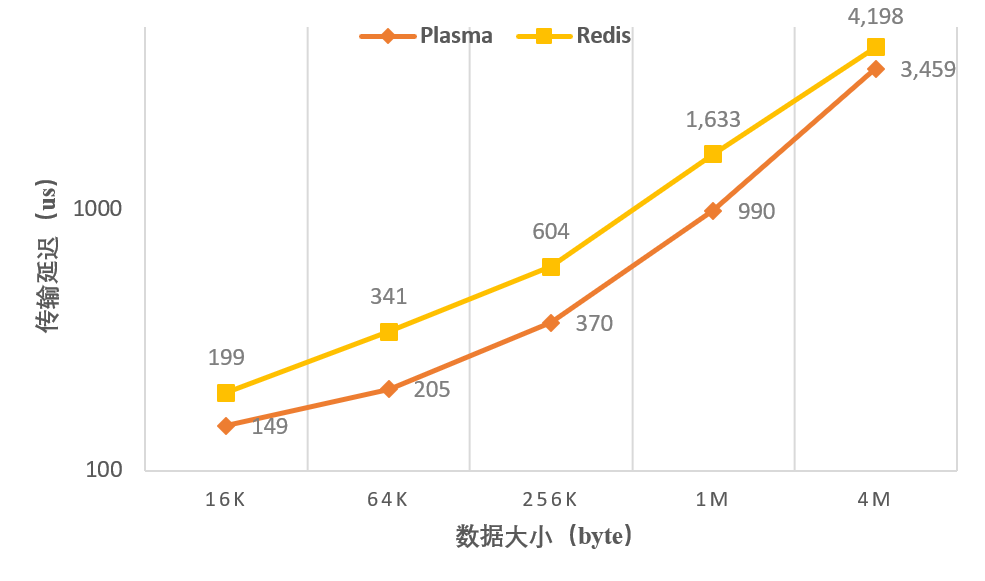
\includegraphics[width=0.9\textwidth]{image/chap04/redis_big.png}
	\caption{Redis和Plasma(优化后)在大对象上的传输延迟}
	\label{fig:redis_big}
\end{figure}
\newclearpage
\chapter{总结与展望}

\section{本研究工作总结}

在本文的研究中,我们探索了一种在最新的分布式计算框架和现代高性能硬件之间进行适配的性能优化。Plasma作为支撑分布式计算框架Ray的分布式内存管理组件,
在设计上并没有考虑过超算集群独特的硬件特性,特别是支持RDMA通信机制的高速网络,因而无法在超算集群上得到最佳的传输性能。我们首先通过跨节点的性能测试
验证了这一设想,特别是发现了其在大对象传输上存在明显的性能缺陷。

面对Ray产生的大小不一的内存对象,我们利用RDMA设计了一种全面优于原实现的对象传输机制。针对小对象的网络传输,我们基于RDMA双边通信原语,设计了一种
低延迟的对象传输协议。该机制能够让接收方的本地访存操作和网络通信重叠,因此具有更优的传输延迟。此外,针对大对象的网络传输,我们使用RDMA单边通信原语设计了
一种兼具低延迟、高带宽的传输协议。该协议所需的通信次数较双边协议更少,并且实现了零拷贝特性,因此大大提升了Plasma在超算网络上的吞吐能力。我们的优化实现能根据
传输的数据大小从上述两种协议中选取合适的执行。

最后,我们对优化实现在各个大小的数据传输进行了性能测试。我们通过实验确定了混合传输机制的选择参数为32KB。双边协议在小于32KB大小的对象传输上实现了最低的
传输延迟。而对于大于32KB的数据对象,使用单边协议则提供了最优的传输带宽,能在4MB及以上大小的数据上提供接近一个数量级的性能提升。此时的Plasma相比Redis数据库,不仅
提供了分布式内存管理的支撑机制,在单节点上的传输性能依然具有明显优势。

\section{未来工作设想}

本文的工作在没有大幅度变动Plasma代码结构的前提下,实现了显著的性能优化——然而,针对分布式内存对象存储,仍然有很多可以探索的空间:

\begin{enumerate}
	\item 即便是采用了RDMA机制用作对象传输,Plasma管理进程仍依赖Redis事件循环库\cite{ae}
	驱动函数调用。目前来看,这一部分仍未支持RDMA,从而限制了Plasma在多节点上的可扩展性。因此后续可以设计基于RDMA的RPC调用组件进一步重构Plasma,以提升其吞吐能力。
	\item 目前的Plasma实现和Ray的对象管理机制\cite{wang2021ownership}没有做到紧耦合,因而存在协同设计(co-design)的可能性。特别是引入支持RDMA特性的高性能网络后,我们是否能进一步设计:
	适应RDMA高速网络的内存对象管理机制,以及支撑该机制的高性能内存存储组件。
	\item 计算框架Ray面向的计算应用,例如强化学习等,大量地使用高性能计算卡(GPU)。然而,目前的Plasma只支持对主存中的数据对象进行存储和管理,对GPU只能控制使用数量。因此,在RDMA机制的帮助下,我们
	是否能将集群内GPU的内存空间纳入管理,并进一步设计异构内存管理机制,是非常值得研究的话题。
\end{enumerate}
\newclearpage
% %% chapter 4 dataset, network structure, experiment and result
% \chapter{实验与结果}
% \label{cha:experiment}


% \newclearpage

% 结语

% 附录部分
\backmatter
% 参考文献. 因不需要纳入章节目录, 故放入附录部分
% 实际上参考文献是属于论文主体部分
\makereferences

% 附录
% {
% \appendix
% \include{docs/appendix1}
% \newclearpage
% }

%%
% 致谢
% 谢辞应以简短的文字对课题研究与论文撰写过程中曾直接给予帮助的人员(例如指导教师、答疑教师及其他人员)表示对自己的谢意,这不仅是一种礼貌,也是对他人劳动的尊重,是治学者应当遵循的学术规范。内容限一页。
% modifier: 黄俊杰
% update date: 2017-04-15
%%

\chapter{致谢}

本科四年的时光匆匆而逝。尽管这四年的学习、生活并不总是一帆风顺,但在大学中我建立了成熟的世界观、学到了宝贵的知识,并且获得了
继续探索未知的兴趣、思维和方法——借助毕业设计的过程,这些收获最终凝聚在了本文中。因此,我首先要感谢本文的指导老师肖侬教授。他对本研究
的研究方向、研究内容和论文写作等方面都有着非常深入的见解。在肖老师的辅导下,我才能顺利地完成本次设计,并将其总结为论文。

在四年求学的道路上,还有很多老师、同学给予了我帮助。虽不能一一列举,但我非常感谢他们。我要特别感谢超算中心的陈志广老师、黄聃老师,他们用心地指导着超算队的比赛和日常运营;黄聃老师
还在研究上给予了我很多指导,让我产生了进一步研究的兴趣和动力。此外,我要感谢中山大学超算队的学长和队员们,超算队提供给我学习前沿知识、参与系统领域竞赛的机会,
丰富了我的本科生涯。最后,我要感谢我的家人们,他们的默默支持是我前进的最大动力。

\vskip 108pt
\begin{flushright}
	兰靖\makebox[1cm]{} \\
	\today
\end{flushright}

    % 致谢
\newclearpage


% \makeGrade      % 成绩评定记录表
\end{document}

